\documentclass[10pt, onecolumn]{article}
\usepackage[utf8]{inputenc}

\usepackage{siunitx}
\usepackage{graphicx}
\usepackage{float}
\usepackage{placeins}
\usepackage{adjustbox}
\usepackage{multirow}
\usepackage[ruled,vlined,linesnumbered]{algorithm2e}
\usepackage{tablefootnote}
\usepackage{mathtools}
\usepackage[margin=0.75in]{geometry} %This is for all the margins

\def\@maketitle{%
  \null
  \vskip 2em%
  \begin{center}%
  \let \footnote \thanks
    {\LARGE \@title \par}%
    \vskip 1.5em%
    {\large
      \lineskip .5em%
      \begin{tabular}[t]{c}% <------
        \@author%            <------ Authors
      \end{tabular}\par}%    <------
    \vskip 1em%
  %  {\large \@date}%
  \end{center}%
  \par
  \vskip 1.5em}

\date{18/03/2019}

\title{\vspace{-2.2cm} \textbf{ELEN4020A: Data Intensive Computing \\ Laboratory Exercise 2}}
\author{\begin{tabular}{ll}
  Lynch Mwaniki & 1043475 \\
  Madimetja Sethosa & 1076467 \\
  Teboho Matsheke & 1157717 \\
\end{tabular}
 }

\begin{document}
%\centering

\maketitle
\thispagestyle{empty}\pagestyle{empty}
\vspace{-8mm}

\section{In-Place Matrix Transposition}
%
In this lab, three different In-place matrix transposition algorithms are implemented and tested against each other: naive approach, Diagonal and Block transpose algorithms. The Diagonal and Block transposition algorithms are implemented using Pthreads and the OpenMP library. The naive approach is implemented serially and using threading by implementing it using the OpenMP library.
%
\section{Basic Algorithm}
%
This algorithm uses two nested for loops to transpose a 2D matrix. The outer and inner loops are used to iterate through the rows and columns of the matrix respectively. They iterate along the main diagonal. Each value is swapped with its corresponding transposed location, $A[i, j]$ with $A[j, i]$. This iteration only needs to be go through either the top or bottom triangular half of the matrix.
%
\begin{figure}[H]
    \centering
    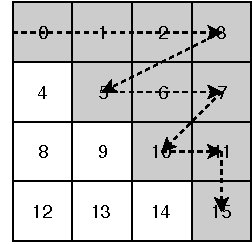
\includegraphics{Documentation/TriangularTraversal.pdf}
    \caption{Traversal of elements in Upper Triangle of a 4x4 Matrix}
    \label{fig:TriangularTraversal}
\end{figure}
%
\section{OpenMP Naive Algorithm}
%
This is a low level improvement of the basic algorithm. The OpenMP \emph{\#pragma} directives are used to parallelize the two nested for loops. The outer loop is used to iterate along the matrix's rows and the inner loop iterates along the columns. 
%
\section{Diagonal Transpose Algorithm}
%
This algorithm transposes the matrix elements by traversing along the matrix diagonal. As with the basic algorithm, each value is swapped with its corresponding transposed location, A[i, j] with A[j, i]. The OpenMP and Pthread methods were implemented and are discussed in the sections that follow. 
%
\subsection{Pthreads}
%
When implementing Pthreads for the Diagonal algorithm, we define a struct named \emph{ThreadDataDiagonal}, with the following properties: diagonal Index, pointer to the matrix, and an ID. We then define or set the number of threads to be used. In order to keep track of the row and column to be transposed, a global variable, nextDiagonal, is defined.

\noindent Each thread's diagonal index property is used to iterate through the columns, of the row associated to the diagonal, of the matrix and transpose the corresponding elements. Upon completion, a \emph{Pthread Mutex Lock} section is created, whereby, if a thread's diagonal index is less than size of the matrix, $N-1$, it is set to nextDiagonal, thereafter, nextDiagonal is incremented by one. Otherwise, the thread diagonal index is set to $N-1$ at which point the thread will exit. The pseudo code for this algorithm can be found in Appendix\,\ref{App:Apendix} Algorithm\,\ref{Alg:PthreadDiagonalTrans}.
%
\subsection{OpenMP}
%
This implementation follows from the basic algorithm. In that it uses two nested for loops to transpose a 2D matrix. In this implementation the OpenMP \emph{\#pragma} directives are used to parallelize the for loop iterations. The outer loop is used to iterate along the matrix's diagonals and the inner loop is used to iterate along the columns. The two nested for loops are enclosed in a parallel section with a pointer to the matrix as shared and the indexing for the diagonal index variable made private. The outer for loop is parallelized with a schedule. The parameters assigned to the schedule is \emph{kind = dynamic} and a \emph{chunk size} = 10. These mean that each thread is given a 10 rows to iterate through. A \emph{nowait} directive is also included, thus allowing a thread to receive the next chunk of indices without waiting for the other threads.
%
\section{Block Transpose Algorithm}
%
The Block Transpose Algorithm consists of three steps. The first step requires a matrix to be divided into blocks of a specified size. The second step involves transposing the elements in the blocks. The last step requires the blocks to be swapped except those on the diagonal. For this lab, a block size of 2x2 was chosen for the block transposition algorithms to use. Figure \ref{fig:BlockDecomposition} shows how a 8x8 matrix is decomposed into 2x2 blocks, which are just sub matrices of size 2x2. The algorithms implemented make use of 2D indexing to assign blocks to threads and represent the 2D input matrices as 1-Dimensional arrays. The 2D indexes of the blocks are mapped to the corresponding 1D indices using the \emph{blockElementsIndex} function which can be seen in Appendix\,\ref{App:Apendix} Algorithm\,\ref{Alg:blockElementsIndex}. The swapping of the blocks is implemented in \emph{swapBlocks} which can be found in Appendix\,\ref{App:Apendix} Algorithm\,\ref{Alg:swapBlocks}.
%
\begin{figure}[H]
    \centering
    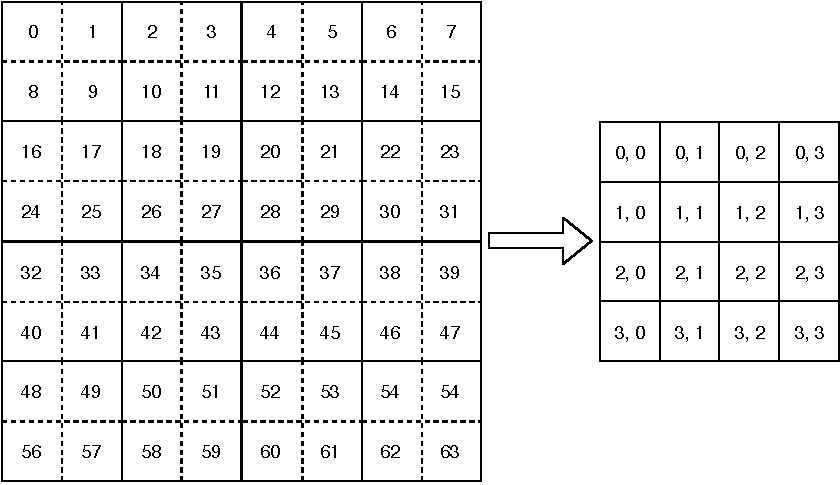
\includegraphics[scale=0.7]{Documentation/BlockDecomposition.pdf}
    \caption{Figure showing a 8x8 matrix decomposed into 2x2 blocks}
    \label{fig:BlockDecomposition}
\end{figure}
%
\subsection{Pthreads}
%
The block transposition algorithms were implemented using the \emph{pthread} library. Two different approaches were implemented and are discussed in the sections that follow.
%
\subsubsection{Algorithm 1}
%
This algorithm performs block transposition by traversing through the upper triangle of a matrix, as shown in Figure\,\ref{fig:TriangularTraversal}. When creating the threads a struct called \emph{ThreadDataBlock} is generated, with the following members: ID, row, column, matrix size and a pointer to the matrix, and assigned to each thread privately. The row and column are indices indicating the block to be worked on. Each thread is assigned a block along the path being traversed. If a thread is assigned a block on the diagonal, it will only transpose the relevant elements in that block. If a thread is assigned a non-diagonal block, it will transpose the elements in that block, interchange the indices, A[i, j] to A[j, i], and swap the corresponding block and finally swap the blocks. Once a thread has completed those steps, a \emph{Pthread\,Mutex\,Lock} section is reached.\\

\noindent This section is needed to update two shared global variables named, \emph{next\_block\_diagonal} and \emph{next\_block\_column}. These variables contain the row and column of the next block that needs to be operated on. The thread saves $\emph{row} = \emph{next\_block\_diagonal}$ and $\emph{column} = \emph{next\_block\_column}$. After the thread saves the information, checks are performed to update the global indexing variables. This section checks that once the \emph{next\_block\_column} reaches the boundary, of the 2D matrix representing the blocks, the \emph{next\_block\_diagonal} is incremented by one and the \emph{next\_block\_column} is set as the value in \emph{next\_block\_diagonal}. The mutex is unlocked and the values row and column values for the thread are checked for boundary conditions. If the row and column received is equal to $matrix\_size - 1$, the thread will exit. The pseudo code code for this algorithm can be found in Appendix\,\ref{App:Apendix} Algorithm\,\ref{Alg:PThreadBlockAlgorithm1}.
%
\subsubsection{Algorithm 2}
%
\begin{figure}[H]
    \centering
    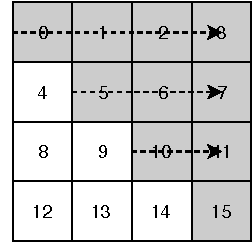
\includegraphics{Documentation/BlockAlgorithm2ThreadAllocation.pdf}
    \caption{Allocation of Blocks to Threads as chunks}
    \label{fig:BlockAlgorithm2ThreadAllocation}
\end{figure}
%
Similar to Algorithm 1, this algorithm traverses the upper triangle of the matrix, but instead of traversing the blocks lineally, they are traversed in a parallel format as shown in Figure \ref{fig:BlockAlgorithm2ThreadAllocation}. Threads are created and each is assigned to a row starting from the diagonal block. If the block assigned to the thread is on the diagonal, then the block is only transposed, else the adjacent block is calculated, transposed and then swapped. The first thread to finish the row will lock the global variable \emph{diag\_index}, copy its value and update it. For a more logical flow of the algorithm, the pseudo code is provided in Appendix\,\ref{App:Apendix} Algorithm\,\ref{Alg:OpenMPBlockAlgorithm2}. 
\subsection{OpenMP block}
%
This implementation follows that of pthread algorithm 2. It makes use of two nested for loops to transpose a 2D matrix. The first for loop is for traversing the diagonal index, where else the second on is for traversing the blocks in each row. The algorithm makes use of \emph{\#progma omp parallel} with the indices of the two for loops being private. The for loop is made parallel with the schedule set to dynamic, this makes sure that each thread executes a chunk of iterations and then requires another chunk of iteration until there is no chunk remaining. The pseudo code is provided in Appendix\,\ref{App:Apendix},\ref{Alg:OpenMPBlockAlgorithm2}.
%
%
\section{Performance Comparison of different algorithms}
The seven algorithms implemented were run on matrix sizes N = 128, 1024, 2048, and 4096. The threaded algorithms were run on each size using 4 threads and 8 threads to gauge the performance of the algorithms. The algorithms were run on a desktop computer with the following specs: an Intel Core i7-6700 CPU with 8\,cores running at 3.40\,GHz and 8\,GB DDR3\,RAM. No other programs were open to ensure that no other known process will slow down the algorithms. Ideally, the algorithms should have been run on a Linux machine with no desktop environment, but this was not available to the group. The results of the implemented algorithms can be seen in Table\,\ref{tbl:Results4Threads}\,-\,\ref{tbl:ResultBasic}.
%
\begin{table}[H]
    \vspace{-0.5cm}
    \centering
    \caption{Results showing time taken to compute algorithms with 4 threads}
    \label{tbl:Results4Threads}
    \begin{tabular}{|l|l|l|l|l|l|l|l|}
    \hline
    \multicolumn{7}{|c|}{\textbf{No. of threads = 4}} \\ \hline
    \multirow{2}{*}{\textbf{$N_0$ = $N_1$}} & \multicolumn{3}{c|}{\textbf{Pthreads}} & \multicolumn{3}{c|}{\textbf{OpenMP}} \\ \cline{2-7} 
    & \textbf{Diagonal} & \textbf{Blocked 1} & \textbf{Blocked 2} & \textbf{Naive} & \textbf{Diagonal} & \textbf{Blocked} \\ \hline
    \textbf{128}  &0.001081  &0.002200  &0.000658  &0.000483  &0.000275  &0.000668  \\ \hline
    \textbf{1024} &0.004056  &0.020829  &0.004910  &0.005325  &0.002941  &0.006797  \\ \hline
    \textbf{2048} &0.020492  &0.027299  &0.028489  &0.031684  &0.021544  &0.032312  \\ \hline
    \textbf{4096} &0.094026  &0.111373  &0.127449  &0.211720  &0.128334  &0.145914  \\ \hline
    \end{tabular}
\end{table}
%
\begin{table}[H]
    \vspace{-0.5cm}
    \centering
    \caption{Results showing time taken to compute algorithms with 8 threads}
    \label{tbl:Results8Threads}
    \begin{tabular}{|l|l|l|l|l|l|l|l|}
    \hline
     \multicolumn{7}{|c|}{\textbf{No. of threads = 8}} \\ \hline
    \multirow{2}{*}{\textbf{$N_0$ = $N_1$}} & \multicolumn{3}{c|}{\textbf{Pthreads}} & \multicolumn{3}{c|}{\textbf{OpenMP}} \\ \cline{2-7} 
    & \textbf{Diagonal} & \textbf{Blocked 1} & \textbf{Blocked 2} & \textbf{Naive} & \textbf{Diagonal} & \textbf{Blocked} \\ \hline
    \textbf{128}  &0.001106  &0.003101  &0.000669  &0.000671  &0.000155  &0.000489  \\ \hline
    \textbf{1024} &0.002545  &0.023252  &0.003740  &0.004816  &0.002402  &0.004610  \\ \hline
    \textbf{2048} &0.016938  &0.029786  &0.017196  &0.024770  &0.020085  &0.022922  \\ \hline
    \textbf{4096} &0.081811  &0.118155  &0.073397  &0.133002  &0.115294  &0.093971  \\ \hline
    \end{tabular}
\end{table}
%
\begin{table}[H]
    \vspace{-0.5cm}
    \centering
    \caption{Results showing time taken to compute the Basic algorithm}
    \label{tbl:ResultBasic}
    \begin{tabular}{|c|c|}
    \hline
    $N_0$ = $N_1$ & Basic \\ \hline
    \textbf{128}        &0.000320       \\ \hline
    \textbf{1024}       &0.010438       \\ \hline
    \textbf{2048}       &0.079379       \\ \hline
    \textbf{4096}       &0.462447       \\ \hline
    \end{tabular}
\end{table}
\section{Analysis of Results}
%
Generally, the basic algorithm was out performed by all the other types of algorithms that were implemented. In table \ref{tbl:Results4Threads} where 4 threads were used for both the openMP and pthread methods, the diagonal algorithm performed better for the both implementations except for N\= 4096 (whereby the block algorithms performed better).  
%
\section{Conclusion}
%
This report detailed three different matrix transposition algorithms implemented in the C programming language namely: Basic or naive approach, Diagonal and Block Transpose algorithms. The Diagonal and Block transposition algorithms were threaded and implemented using two different threading libraries namely: Pthreads and OpenMP. The Naive approach was also threaded using OpenMP. The algorithms were timed and the results were analyzed. It was discovered that the pthreads algorithm 2 out performs the rest of the algorithms for N $>$ x. 
%
\clearpage
\appendix

\section{Pseudo code}
\label{App:Apendix}
\subsection{allocateMatrix}
    \begin{algorithm}[H]
        \label{Alg:allocateMatrix}
        \caption{Allocate Matrix in Memory}
        \KwResult{Integer pointer, pointing to first element of matrix.}
        \SetKwInOut{Input}{Input}\SetKwInOut{Output}{Output}
        \Input{Total Number of Elements}
        result\_ptr = (int*)calloc(number\_of\_elements, sizeof(int)) \\
        \Return result\_ptr
    \end{algorithm}
%
\subsection{getElementLocation2D}

    \begin{algorithm}[H]
        \label{Alg:getElementLocation2D}
        \caption{Get Location of Element in 2D matrix when represented as 1D Array}
        \KwResult{Integer containing position of element in 1D matrix}
        \SetKwInOut{Input}{Input}\SetKwInOut{Output}{Output}
        \Input{1D Array containing indexes}
        \Input{Dimension N}
        row = index[0]\\
        column = index[1]\\
        \Return $(row*N)+column$
    \end{algorithm}
 % 
\subsection{retrieveElement2D}

    \begin{algorithm}[H]
        \label{Alg:retrieveElement2D}
        \caption{Retrieve Element from 2D matrix}
        \KwResult{Integer value of the element in the 2D matrix co-ordinates.}
        \SetKwInOut{Input}{Input}\SetKwInOut{Output}{Output}
        \Input{Pointer to matrix, 1D Array containing indexes}
        \Input{Dimension N}
        \Return $*(matrix\_ptr + getElementLocation2D(indexes, N))$
    \end{algorithm}
%
 % 
\subsection{blockElementsIndex}

    \begin{algorithm}[H]
        \label{Alg:blockElementsIndex}
        \caption{Retrieve block Elements indices}
        \KwResult{4 index values of a block in the matrix}
        \SetKwInOut{Input}{Input}\SetKwInOut{Output}{Output}
        \Input{blockIndex, Dimension N}
        Num\_Blocks = N/2\\
        *blockElemIndex =  (blockIndex*2)+ ((int)(blockIndex/Num\_Blocks))*N;\\
	    blockElemIndex[1]=*blockElemIndex+1; \\
	    blockElemIndex[2]=*blockElemIndex+N;\\
	    blockElemIndex[3]=*blockElemIndex+(N+1);\\
        \Return $blockElemIndex$
    \end{algorithm}
%
 % 
\subsection{swapBlocks}

    \begin{algorithm}[H]
        \label{Alg:swapBlocks}
        \caption{transpose two blocks}
        \KwResult{block transposed *matrix}
        \SetKwInOut{Input}{Input}\SetKwInOut{Output}{Output}
        \Input{*matrix, *blockA, *blockB}
        swapElements(matrix+indexBlockA[0], matrix+indexBlockB[0]);\\
	swapElements(matrix+indexBlockA[1], matrix+indexBlockB[1]);\\
	swapElements(matrix+indexBlockA[2], matrix+indexBlockB[2]);\\
	swapElements(matrix+indexBlockA[3], matrix+indexBlockB[3]);\\
    \end{algorithm}
%
\subsection{Basic Algorithm}

%
%
\begin{algorithm}[H]
    \label{Alg:BasicAlgorithm}
    \caption{Transpose a square 2D Matrix using Naive Approach in Serial execution}
    \KwResult{A 2D square transposed matrix}
    \SetKwInOut{Input}{Input}\SetKwInOut{Output}{Output}
    \Input{Pointer to matrix}
    \Input{Matrix Size N}
    \For{ i = 0 to N - 1}
    {
        \For{ j = i to N-1}
        {
            temp = matrix element indexed at i and j \\
            matrix element at i and j position = matrix element indexed at j and i position\\
            matrix element indexed at j and i position = temp
        }
    }
\end{algorithm}
%
\subsection{OpenMP Naive Transpose Algorithm}

%
\begin{algorithm}[H]
    \label{Alg:OpenMPNaiveAlgorithm}
    \caption{Transpose a square 2D Matrix using Naive Approach in Parallel execution}
    \KwResult{A 2D square transposed matrix}
    \SetKwInOut{Input}{Input}\SetKwInOut{Output}{Output}
    \Input{Pointer to matrix}
    \Input{Matrix Size N}
    Set number of threads for OpenMP\\
    Create variables i, j and temp\\
    \#pragma omp parallel shared(matrix) private(temp, i, j)\\
    \#pragma omp for schedule(dynamic) nowait\\
    \For{ i = 0 to N - 1}
    {
        \For{ j = i to N-1}
        {
            temp = matrix element indexed at i and j \\
            matrix element at i and j position = matrix element indexed at j and i position \\
            matrix element indexed at j and i position = temp
        }
    }
\end{algorithm}
%
\subsection{OpenMP Diagonal Transpose Algorithm}

%
\begin{algorithm}[H]
    \label{Alg:OpenMPDiagonalAlgorithm}
    \caption{Transpose a square 2D Matrix using Naive Approach in Parallel execution}
    \KwResult{A 2D square transposed matrix}
    \SetKwInOut{Input}{Input}\SetKwInOut{Output}{Output}
    \Input{Pointer to matrix}
    \Input{Matrix Size N}
    Set number of threads for OpenMP\\
    Create variables diagonalIndex, chunk\_size and temp\\
    Assign chunk\_size to 10 \\
    \#pragma omp parallel shared(matrix) private(diagonalIndex, temp)\\
    \#pragma omp for schedule(dynamic, chunk\_size) nowait\\
    \For{ diagonalIndex = 0 to N - 2}
    {
        \For{ int column = diagonalIndex + 1 to N-1}
        {
            temp = matrix element indexed at diagonalIndex and column \\
            matrix element at [diagonalIndex, column] position = matrix element indexed at [column,  diagonalIndex] position \\
            matrix element indexed at [column, diagonalIndex] position = temp
        }
    }
\end{algorithm}
%
\subsection{OpenMP Block Transpose Algorithm}
%
\begin{algorithm}[H]
   \label{Alg:OpenMPBlockAlgorithm2}
    \caption{Transpose a square 2D Matrix using Block Transpose Algorithm}
    \KwResult{A 2D square transposed matrix}
    \SetKwInOut{Input}{Input}\SetKwInOut{Output}{Output}
    set number of threads for Pthreads\\
    
    \textbf{in main:} \\
    Allocate memory for 2D matrix of size N and fill with random integers \\
    Calculate the number of blocks (N\_blocks)\\
    \ForEach{thread}
    {   
       \#pragma omp parallel private(i,j)
        {
        
            \#pragma omp for schedule(dynamic)
            {
                \For{ j = diagIndex to N\_blocks}
                {
                    temp = matrix element indexed at diagIndex and j \\
                    get blockA element indices using the blockElementsIndex function\\
                    transpose the elements in blockA\\
                    \If{j!=diagIndex}{
                        temp = matrix element indexed at j and diagIndex\\
                        get blockB element indices using the blockElementsIndex function\\
                        transpose the elements in blockB\\
                        
                        transpose blockA and blockB using the swapBlocks() function.
                    }
            }
            }

        }
    }
\end{algorithm}
%
\subsection{Pthread Diagonal Transpose Algorithm}
%
\begin{algorithm}[H]
    \label{Alg:PthreadDiagonalTrans}
    \caption{Transpose a square 2D Matrix using Diagonal Algorithm}
    \KwResult{A 2D square transposed matrix}
    \SetKwInOut{Input}{Input}\SetKwInOut{Output}{Output}
    Set number of threads for Pthreads.\\
    Create global variable \textbf{nextDiagonal} and set it to number of threads. \\
    struct ThreadData[ int* matrix; int diagIndex;] \\
    
    \textbf{in main:} \\
    Allocate memory for 2D matrix of size N and fill with random integers. \\
    Create 1D matrix of size number of Pthreads for storing structs of type ThreadData. \\
    Create Pthread threads with number assigned above.\\
    
    \ForEach{thread}
    {   
        Assign threadData's matrix pointer to the 2D matrix created earlier.\\
        Assign threadData's diagIndex to the ID of the thread being created.\\
        \While{true}
        {
            \For{int column = diagIndex + 1 to N - 1}
            {
                temp = matrix element indexed at diagonalIndex and column \\
                matrix element at [diagonalIndex, column] position = matrix element indexed at [column,  diagonalIndex] position \\
                matrix element indexed at [column, diagonalIndex] position = temp
            }
            
            Mutex Lock\\
            %
            \If{nextDiagonal $<=$ N - 1}
            {
                diagIndex = nextDiagonal\\
                Increment nextDiagonal by 1.
                }
            \Else{ diagIndex = N - 1 }
            %
            Mutex Unlock\\
            
            \If{diagIndex == N - 1}{ break from while loop}
        }
        exit pthread
    }
    
    \ForEach{thread}
    {
        Join thread and wait for other threads to exit and join
    }
\end{algorithm}
%
\clearpage
\subsection{Pthread Block Transpose Algorithm 1}
%
\begin{algorithm}[H]
   \label{Alg:computeNextBlock}
   \caption{Compute next block to be worked on in Algorithm \ref{Alg:PThreadBlockAlgorithm1}}
   \KwResult{The row and column of the next block to be transposed.}
   \SetKwInOut{Input}{Input}\SetKwInOut{Output}{Output}
   \Input{N = size of input matrix}
   Compute size of matrix of blocks: $N\_block = N/2$\\
   Increment next\_block\_column by 1. \\
   \If{next\_block\_column \textbf{mod} N\_block \textbf{equals} 0 \textbf{and} next\_block\_column \textbf{not equal to} 0}
   {
        Increment next\_block\_diagonal by 1.\\
        Set next\_block\_column = next\_block\_diagonal.
   }
   
   \If{next\_block\_column $>=$ N\_block \textbf{and} next\_block\_diagonal $>=$ N\_block}
   {
        Set next\_block\_diagonal = N\_block. \\
        Set next\_block\_column = N\_block.
   }
   \Return
\end{algorithm}
%
\begin{algorithm}[H]
   \label{Alg:PThreadBlockAlgorithm1}
    \caption{Transpose a square 2D Matrix using Block Transpose Algorithm}
    \KwResult{A 2D square transposed matrix.}
    \SetKwInOut{Input}{Input}\SetKwInOut{Output}{Output}
    Set number of threads for Pthreads.\\
    Create global variables \textbf{next\_block\_column}, \textbf{next\_block\_diagonal}. \\
    Create pthread mutex \textbf{computeNextBlockLock}. \\
    struct ThreadDataBlock[ int* matrix; int row, column, N;] \\
    \textbf{in main:} \\
    Allocate memory for 2D matrix of size N and fill with random integers. \\
    Create 1D matrix of the size of number Pthreads for storing structs of type ThreadDataBlock. \\
    Create pthread threads with number assigned above.\\
    \ForEach{thread}
    {   
        Assign threadDataBlock's matrix pointer to the 2D matrix created earlier.\\
        Assign threadDataBlock's row to next\_block\_diagonal.\\
        Assign threadDataBlock's column to next\_block\_column.\\
        Call computeNextBlock function.\\
        Calculate the number of blocks (N\_blocks).\\
        \While{true}
        {
            Set index[2] = [threadDataBlock.row, threadDataBlock.column]. \\
            Get blockA element indices at block located at \emph{index} using the blockElementsIndex function.\\
            Transpose the elements in blockA.\\
            \If{index[0] \textbf{not equal to} index[1]}
            {       
                Set index[0] = threadDataBlock.column\\ 
                Set index[1] = threadDataBlock.row \\
                Get blockB element indices at block located at \emph{index} using the blockElementsIndex function.\\
                Transpose the elements in blockB.\\
                Transpose blockB using the swapBlocks() function.
            }
            
            \emph{computeNextBlockLock} Lock\\
            %
            Assign threadDataBlock's row to next\_block\_diagonal.\\
            Assign threadDataBlock's column to next\_block\_column.\\
            Call computeNextBlock function.\\
            %
            \emph{computeNextBlockLock} Unlock\\
            
            \If{threadDataBlock.row == N\_block \textbf{and} threadDataBlock.column == N\_block}
            { break from while loop}
        }
        Exit pthread
    }
    \ForEach{thread}
    {
        Join thread and wait for other threads to exit and join
    }
\end{algorithm}
%
\subsection{Pthread Block Transpose Algorithm 2}
%

\begin{algorithm}[H]
   \label{Alg:PThreadBlockAlgorithm2}
    \caption{Transpose a square 2D Matrix using Block Transpose Algorithm}
    \KwResult{A 2D square transposed matrix}
    \SetKwInOut{Input}{Input}\SetKwInOut{Output}{Output}
    set number of threads for Pthreads\\
    create global variable \textbf{nextDiagBlock} \\
    struct ThreadData[ int* matrix; int diagIndex;] \\
    
    \textbf{in main:} \\
    Allocate memory for 2D matrix of size N and fill with random integers \\
    Create 1D matrix of the size of number Pthreads for storing structs of type ThreadData \\
    Create pthread threads with number assigned above.\\
    Calculate the number of blocks (N\_blocks)\\
    \ForEach{thread}
    {   
        Assign threadData's matrix pointer to the 2D matrix created earlier.\\
        Assign threadData's diagIndex to the ID of the thread being created.\\
        \While{true}
        {
            \For{ j = diagIndex to N\_blocks}
            {
                temp = matrix element indexed at diagIndex and j \\
                get blockA element indices using the blockElementsIndex function\\
                transpose the elements in blockA\\
                \If{j!=diagIndex}{
                    temp = matrix element indexed at j and diagIndex\\
                    get blockB element indices using the blockElementsIndex function\\
                    transpose the elements in blockB\\
                    
                    transpose blockA and blockB using the swapBlocks() function.
                }
            }
            
            Mutex Lock\\
            %
            \If{nextDiagBlock $<$ N\_blocks - 1} {diagIndex = nextDiagBlock++;}
            \Else{diagIndex=N\_blocks - 1}
            %
            Mutex Unlock\\
            
            \If{diagIndex == N\_blocks - 1}{ break from while loop}
        }
        exit pthread
    }
    
    \ForEach{thread}
    {
        Join thread and wait for other threads to exit and join
    }
\end{algorithm}
%
\end{document}